% To add an image or include a .tex file you need to add
% \CWD
% to the relative (to the main document) path.
%
% Example:
% \begin{figure}
%   \centering
%   \includegraphics{\CWD/images/example.pdf}
% \end{figure}

\begin{center}
\textit{Bacon, O Próspero, é reverenciado no reino das capivaras por seu glorioso reinado de paz e progresso, fruto de sua inabalável devoção ao Deboísmo,
religião que hoje é seguida por mais de 90\% dos habitantes da Bacônia. O Deboismo prega que todos seus seguidores devem ficar o máximo possível
de boa na lagoa, evitando assim os estresses e aflições que diminuem a qualidade de vida e geram o caos social. Além disso, ele patrocina várias festas
populares e, certamente, as Festas da Cheia (para celebrar as chuvas de fim de ano) e suas árvores mágicas são as mais incríveis de todas.}
\end{center}

\begin{figure}[H]
  \centering
  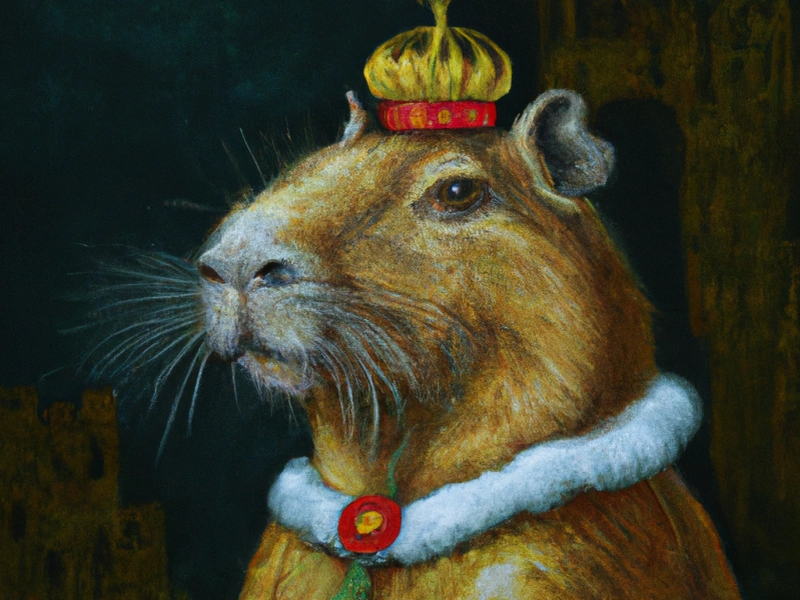
\includegraphics[width=7cm]{\CWD/capivara.png}
\end{figure}

Árvores mágicas possuem luz própria, são enraizadas, e funcionam da seguinte forma:

\begin{itemize}
	\item A árvore inicia-se com todos os vértices apagados.
	\item Uma sub-árvore inteira pode se acender ou se apagar.
	\item Um vértice interno da árvore está aceso se e somente se todos os seus filhos estão acesos.
\end{itemize}

Além da magia da luz própria, a terceira propriedade também é bem misteriosa. Note que, se a sub-árvore enraizada em $v$ é desligada,
todos os ancestrais de $v$ ligados também devem ser desligados; por outro lado se a sub-árvore de $v$ é ligada, pode ser que tenhamos de ligar o pai de $v$,
se todos seus filhos agora estiverem ligados, e assim sucessivamente.

Na 13ª Festa da Cheia de seu reinado, Bacon, O Próspero, levou seu bisneto, que viria a ser o rei Bacon, O Grafo, para ver a árvore mágica plantada
no palácio. Como todo bom amante da combinátoria, a pequena capivara perguntava incessantemente ao bisavô quantos vértices de uma dada sub-árvore estavam acesos.
Infelizmente, nosso herói não é lá muito bom nessa área, e pediu a você, Grande Maratonista, para o ajudar a responder as perguntas do futuro monarca!

%
% For input, use one of the following
%

\section*{Entrada}

A primeira linha contém um inteiro $1 \leq N \leq 10^5$, o número de vértices da árvore.
As próximas $N-1$ linhas contém as arestas $1 \leq a_i, b_i \leq N$ da árvore. É garantido que as arestas descrevem uma árvore, e a raiz é
o vértice de número $1$.

A próxima linha contém o um inteiro $1 \leq Q \leq 10^5$ que representa o número de eventos presenciados por Bacon, O Próspero.
As próximas $Q$ linhas contém 2 inteiros cada, $t_i, v_i$, em que $t_i \in \{1, 2, 3\}$ define o $i$-ésimo evento e $1 \leq v_i \leq N$ o vértice que enraiza a sub-árvore em questão.
\begin{itemize}
\item Se $t_i = 1$, então a sub-árvore enraizada em $v_i$ se acende.
\item Se $t_i = 2$, a sub-árvore enraizada em $v_i$ se apaga.
\item Se $t_i = 3$, o pequeno Bacon perguntou a seu bisavô quantos vértices na sub-árvore enraizada em $v_i$ (inclusive $v_i$) estavam acesos.
\end{itemize}

%
% For output, use one of the following
%

\section*{Saída}

Para eventos do tipo $3$, imprima o número de vértices acesos na sub-árvore enraizada em $v_i$.

%\sampleio will look for files named sample-n.in and sample-n.sol (where n is 1, 2, 3...)
%in the documents directory and include them as samples.

\section*{Restrições}

\begin{itemize}
\item $1 \leq N, Q \leq 10^5$.
\end{itemize}

\exemplo
